\newgeometry{top=1 in, bottom=1 in, left=1.5 in, right=1.5 in}

\section{Simulering}
Resultaterne fra analysen simuleres med diagrammerne vist i Figur  og Figur . 

\subsection{Simulering af 1. ordens lavpasfilter}

\subsubsection{Simulering af 10 k$\Omega$ }
Figur \ref{1.orden} viser simuleringen af 1. ordens lavpasfilter. På oscilloskopet vises kurveformen for $V_{out}$ og heraf bestemmes tidskonstan for R = 10 k$\Omega$ og R = 100k$\Omega$.
I de to tilfælde bestemmes den maksimale værdi af $V_{out}$
Resultaterne indføres i tabel 1.

\begin{figure}[h]
 \begin{center}
  \includegraphics[height=5cm{P_Fig/figur1}
  \caption{Simulering af 1. ordens lavpasfilter}
  \label{1.orden}
 \end{center}
\end{figure}

tidskonstanten($\tau$) bestemmes ved at først at beregne 

$V_max \cdot 0.63 = V_{\tau}$

Herefter måles tidsforskellen fra $t_0 V$ til $V_{\tau}$

$V_max$ er ud fra figur \ref{10k.50Hz.tau} målt til 4.97 V
$4.97 V \cdot 0.63 = 3.131 V$

tidsforskellen fra $t_0 V$ til $V_{\tau}$ måles til 1.01 ms

\begin{figure}[h]
 \begin{center}
  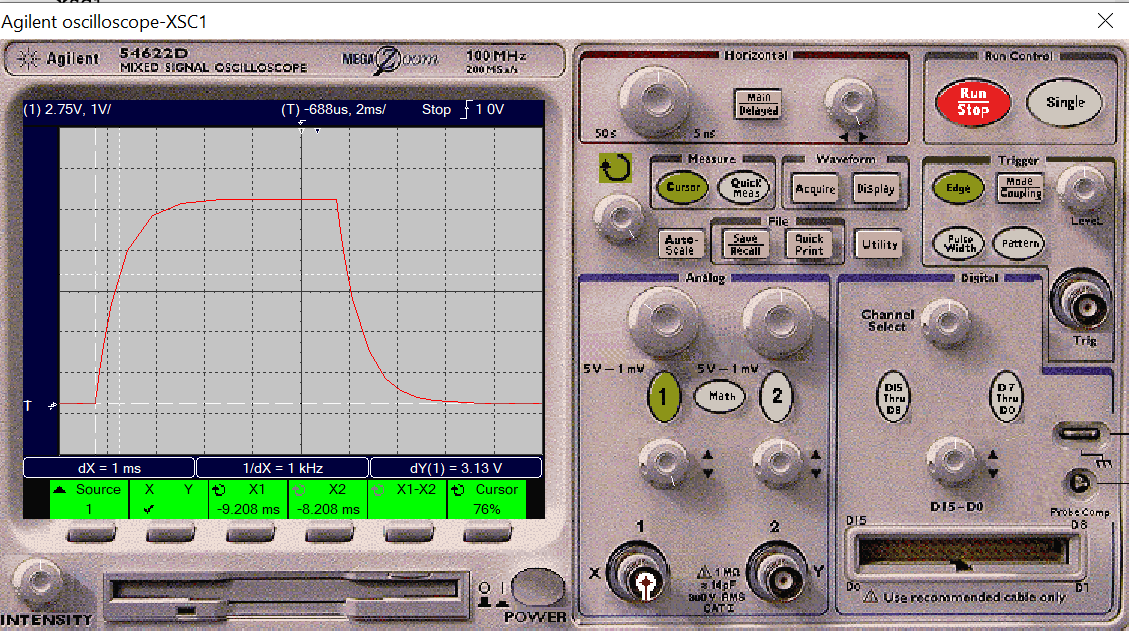
\includegraphics[height=5cm]{P_Fig/figur3.10k.50Hz.tau}
  \caption{måling af $\tau$}
  \label{10k.50Hz.tau}
 \end{center}
\end{figure}

stigetiden($\tau$) bestemmes ved formlen:
$\tau_{90} - \tau_{10} = \delta_{stigetid}$

Ud fra målinger af figur \ref{10k.50Hz.stigetid}
er stigetiden blevet beregnet til

$\tau_{10} = 4.97 V \cdot 0.1 = 0.497 V$
$\tau_{90} = 4.97 V \cdot 0.9 = 4.473 V$

Herefter måles afstanden mellem $\tau_{10}$ til $\tau{90}$ som via figur \ref{10k.50Hz.stigetid} bliver målt til 2.08 ms

\begin{figure}[h]
 \begin{center}
  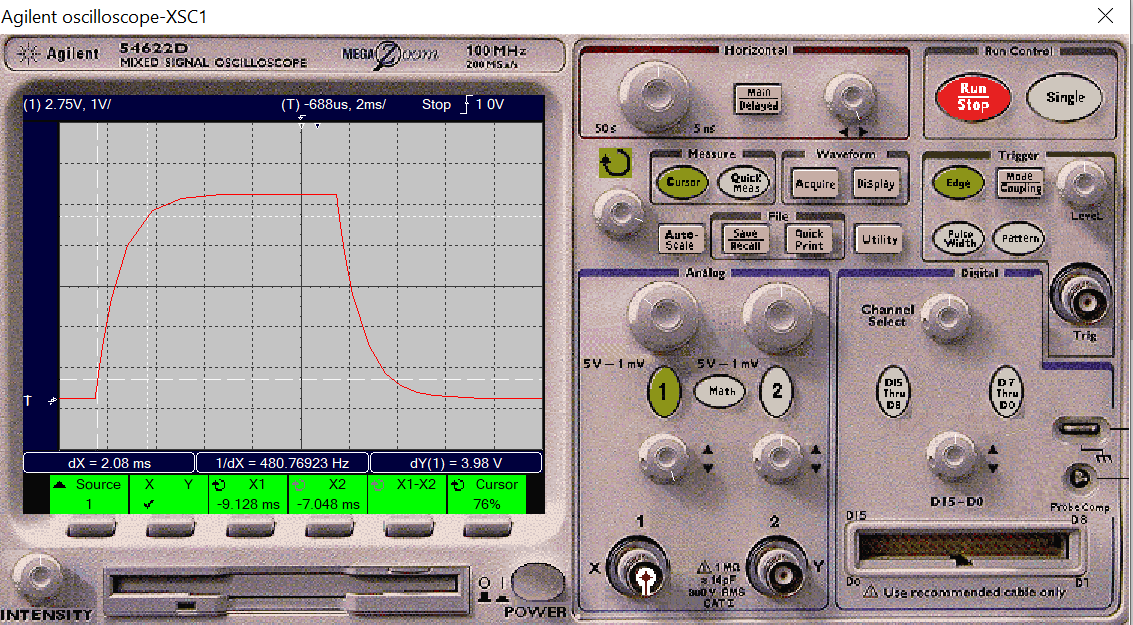
\includegraphics[height=5cm]{P_Fig/figur4.10k.50Hz.stigetid}
  \caption{stigetid}
  \label{10k.50Hz.stigetid}
 \end{center}
\end{figure}

Maksimal spænding bliver målt med formlen
$V_{max} - V_{min}$

Afstanden mellem $V_{max}$ og $V_{min}$ som via figur \ref{10k.50Hz.min.max} måles til 4.97 V

\begin{figure}[h]
 \begin{center}
  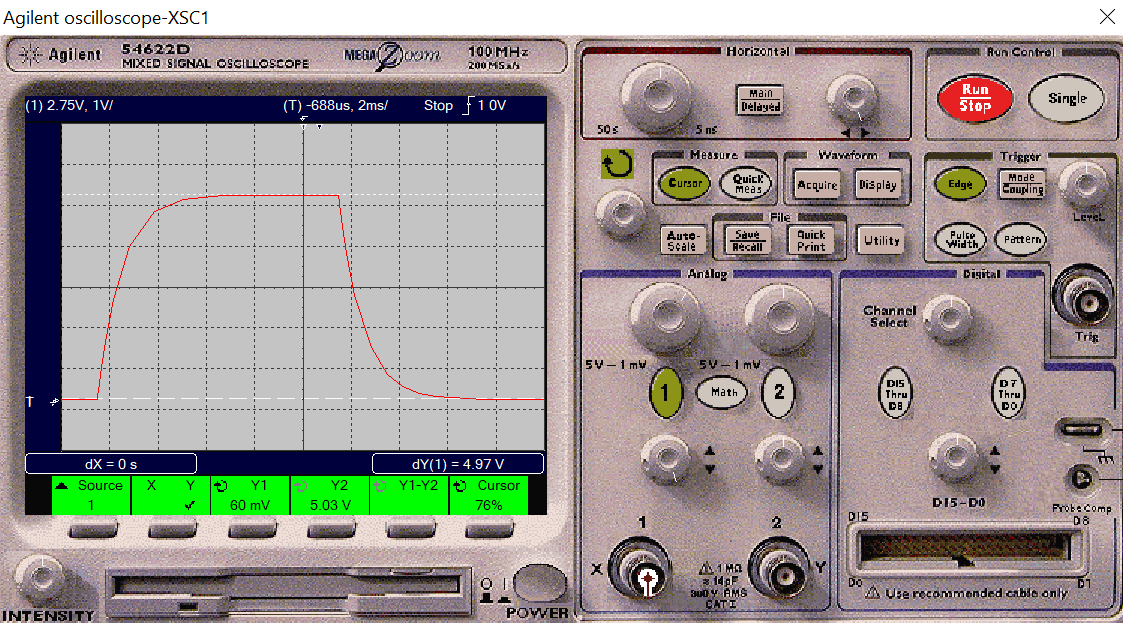
\includegraphics[height=5cm]{P_Fig/figur2.10k.50Hz.min.max}
  \caption{Maksimal spænding}
  \label{10k.50Hz.min.max}
 \end{center}
\end{figure}


\subsubsection{Simulering af 100 k$\Omega$ }
tidskonstanten($\tau$) bestemmes ved at først at beregne 

$V_max \cdot 0.63 = V_{\tau}$

Herefter måles tidsforskellen fra $t_0 V$ til $V_{\tau}$

$V_max$ er ud fra figur \ref{100k.5Hz.tau} målt til 4.96 V
$4.96 V \cdot 0.63 = 3.125 V$

tidsforskellen fra $t_0 V$ til $V_{\tau}$ måles til 10.04 ms

\begin{figure}[h]
 \begin{center}
  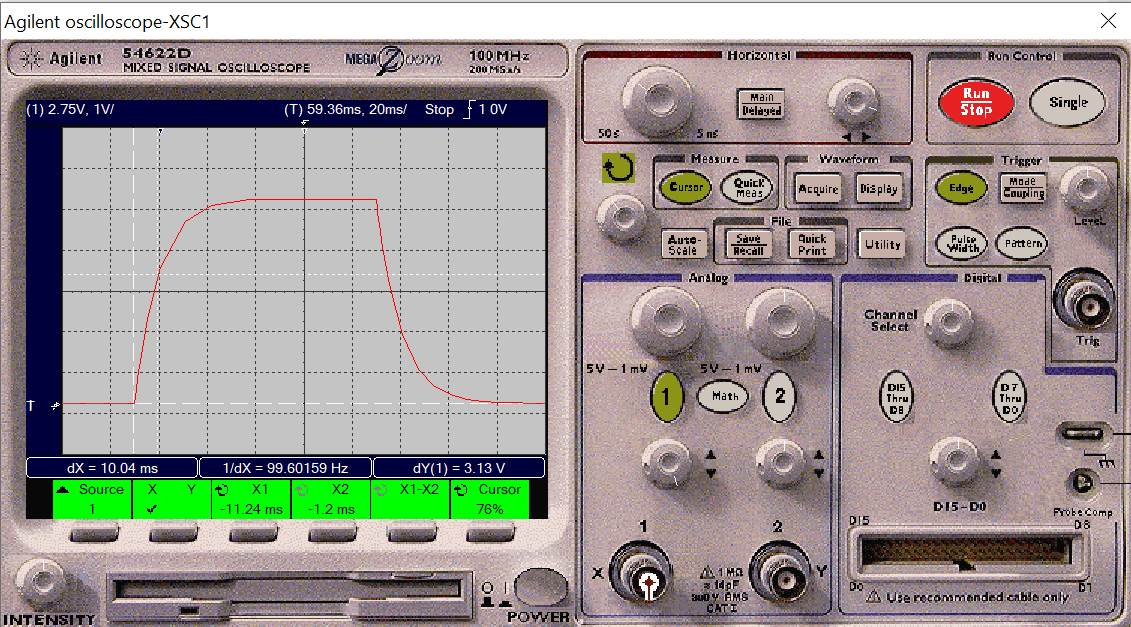
\includegraphics[height=5cm]{P_Fig/figur6.100k.5Hz.tau}
  \caption{måling af $\tau$}
  \label{100k.5Hz.tau}
 \end{center}
\end{figure}

stigetiden($\tau$) bestemmes ved formlen:
$\tau_{90} - \tau_{10} = \delta_{stigetid}$

Ud fra målinger af figur \ref{100k.5Hz.stigetid}
er stigetiden blevet beregnet til

$\tau_{10} = 4.96 V \cdot 0.1 = 0.496 V$
$\tau_{90} = 4.96 V \cdot 0.9 = 4.464 V$

Herefter måles afstanden mellem $\tau_{10} til \tau{90}$ som via figur \ref{100k.5Hz.stigetid} bliver målt til 19.72 ms

\begin{figure}[h]
 \begin{center}
  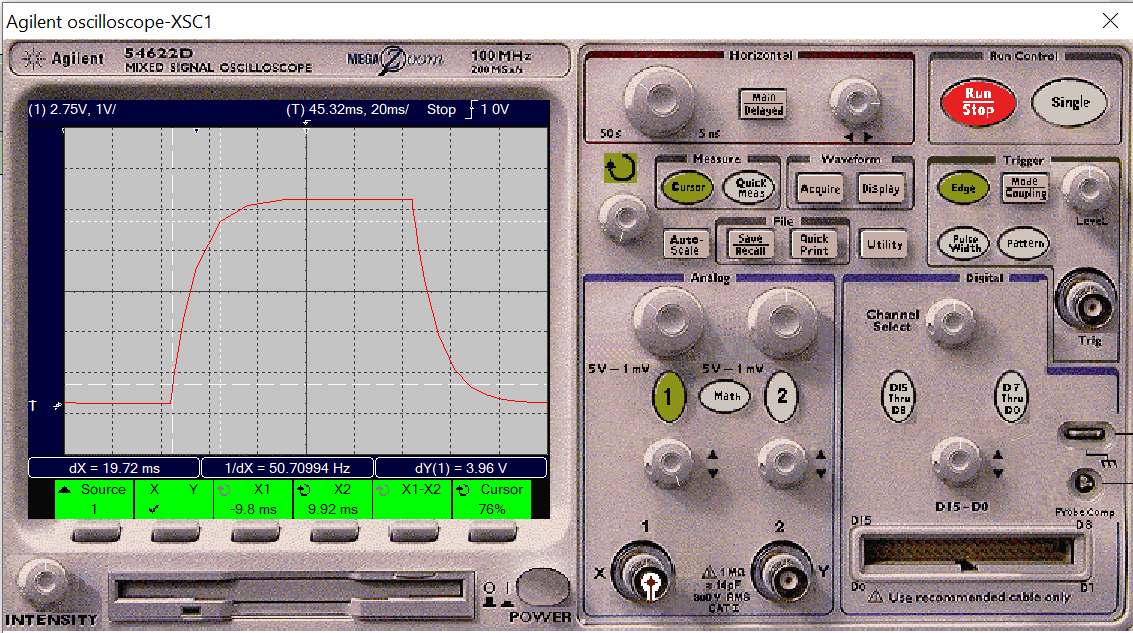
\includegraphics[height=5cm]{P_Fig/figur7.100k.5Hz.stigetid}
  \caption{stigetid}
  \label{100k.5Hz.stigetid}
 \end{center}
\end{figure}

Maksimal spænding bliver målt med formlen
$V_{max} - V_{min}$

Afstanden mellem $V_{max}$ og $V_{min}$ som via figur \ref{100k.5Hz.min.max} måles til 4.96 V

\begin{figure}[h]
 \begin{center}
  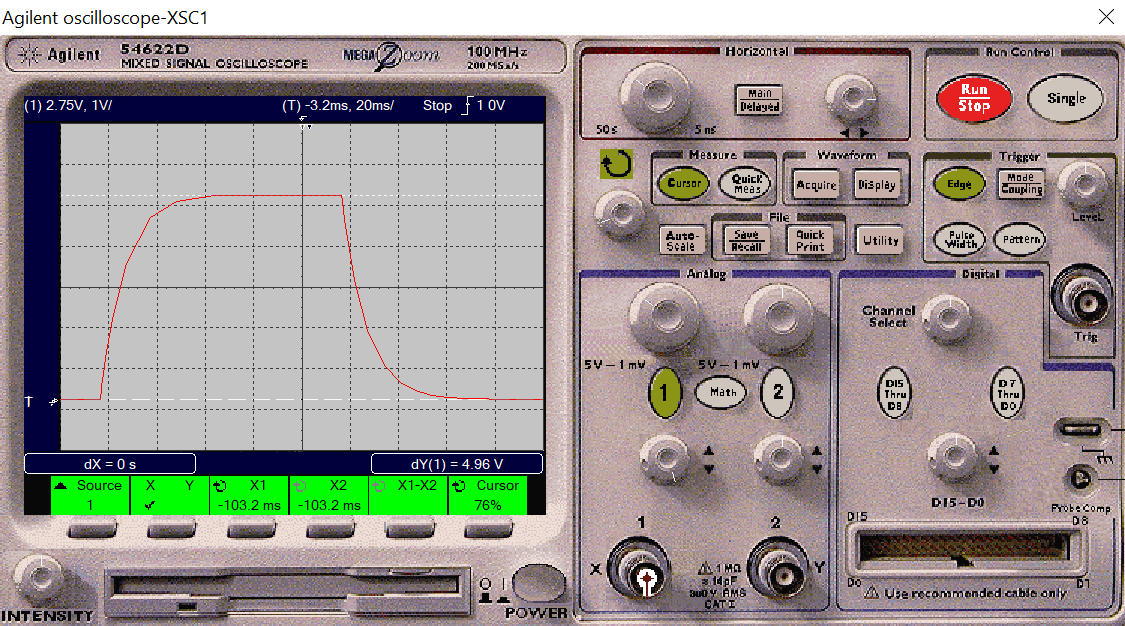
\includegraphics[height=5cm]{P_Fig/figur5.100k.5Hz.min.max}
  \caption{Maksimal spænding}
  \label{100k.5Hz.min.max}
 \end{center}
\end{figure}
